\documentclass{beamer}

\mode<presentation> {
}
\addtobeamertemplate{footline}{\insertframenumber/\inserttotalframenumber}

%\bibliographystyle{abbrvnat}

%\usepackage{comment}
\usepackage{amsmath,amsfonts, amssymb, dsfont, amsthm}
\usepackage{hyperref}
\usepackage{nicematrix}
\usepackage{tabstackengine}
\usepackage{bm}
\usepackage[ruled,algo2e]{algorithm2e}
\usepackage{xfrac}
\usepackage{tikz}
\usepackage{mathabx}
\usepackage{tcolorbox}
\usecolortheme{orchid}


\usepackage[english]{babel}
\usepackage{booktabs} % Allows the use of \toprule, \midrule and \bottomrule in tables
\usepackage{caption}
\usepackage{subcaption}
% \usepackage[round]{natbib}
% \bibliographystyle{abbrvnat}
% \setcitestyle{authoryear,open={(},close={)},citesep={,}}
\usepackage[absolute,overlay]{textpos}
\usepackage{graphicx}
\usepackage{graphics}
\title{\parbox{\linewidth}{
    \centering Zero-inflation in the Multivariate Poisson Lognormal Family}}
\author{Bastien Batardière, François Gindraud, Julien Chiquet and Mahendra Mariadassou}
\date{\today}
\institute{Université Paris-Saclay, AgroParisTech, INRAE, UMR MIA Paris-Saclay, MaIAGE}

\newtheorem{Theorems}{Theorems}[section]
\newtheorem{Assumption}[Theorems]{Assumption}
\newtheorem{prop}[Theorems]{Proposition}
\newtheorem{rem}[Theorems]{Remark}
\newtheorem{cor}[Theorems]{Corollary}
\theoremstyle{remark}
\newtheorem{remark}[Theorems]{Remark}

% \newtheorem{Theorem}{Theorem}[section]
% \newtheorem{prop}[Theorem]{Proposition}

\newcommand*{\colorboxed}{}
\def\colorboxed#1#{%
  \colorboxedAux{#1}%
}
\newcommand*{\colorboxedAux}[3]{%
  % #1: optional argument for color model
  % #2: color specification
  % #3: formula
  \begingroup
    \colorlet{cb@saved}{.}%
    \color#1{#2}%
    \boxed{%
      \color{cb@saved}%
      #3%
    }%
  \endgroup
}


\newcommand{\matr}[1]{\boldsymbol{\mathbf{#1}}}
\newcommand{\indep}{\perp \!\!\! \perp}

\DeclareMathOperator*{\argmax}{\arg\!\max}
\DeclareMathOperator*{\argmin}{\arg\!\min}



\begin{document}
\begin{frame}
    \titlepage
\end{frame}

\begin{frame}
\begin{itemize}
    \item In Single cell analysis, it is usual to deal with high-dimensional count data:
\newline
\vspace{-0.9cm}
 \[
  \boldsymbol{Y} =  \bordermatrix{~  &  &  &  &
                        &   \cr
                      & 12  & 0 & \cdots & 0 &  9  \cr
                     & 2 & 0 & \cdots & 0 & 0  \cr
                     & \vdots &  &  &  & \vdots  \cr
                     & 341 & 5 & \cdots & 1 & 0  \cr
                    }
\]
\item $Y_{ij}$: count of transcript $j$ in cell $i$
\item \textbf{Non-continuous data} $\implies$ Linear Gaussian models do not apply
\item \textbf{High percentage of zeros ($\approx 80\%$)} $\implies$ zero-inflation is needed
\end{itemize}
\end{frame}

\begin{frame}
\begin{itemize}
    \item Dataset:
    \begin{itemize}
        \item $\boldsymbol{Y}: n \times p$ count matrix ( $n \approx p \approx 10^4$)
        \item $\boldsymbol{X}: n\times d $ or $d \times p$ covariates ($d \approx 10$)
    \end{itemize}
    \item Parameter $\theta = \left(\matr B,\matr  \Sigma, \matr \pi\right) $
    \begin{itemize}
        \item $\matr B \in \mathbb R^{d\times p} $ regression coefficient.
        \item $\matr \Sigma \in \mathbb R^{p\times P }$ covariance matrix.
        \item $\matr \pi \in \mathbb R^{n\times p}$ zero-inflation coefficient.
    \end{itemize}
    \item Model:%\vspace{-2.4cm}
% \centering {
% \Large
\begin{align*}
    \mathbf{W_{i}}  & \sim \mathbf{\mathcal{B}}\left(\pi_i\right) \\
    \boldsymbol{Z_{i}} & \sim \mathcal  N\left( \matr X \matr B, \matr \Sigma \right)  \\
    \left(Y_{ij}   \mid Z_{i j}, W_{ij} \right) & \sim \left( 1- W_{ij} \right) \mathcal{P}\left(\exp \left( Z_{i j}\right)\right)
 \end{align*}
 % \par
% }\par
\end{itemize}
\end{frame}
\begin{frame}{Modelling the zero inflation}
    The zero-inflation can take several forms:
 \begin{subequations}
\begin{align*}
\bullet ~ \pi_{ij}  & = \pi \in [0,1]& \text{(non-dependent)}  \\
 \bullet ~ \pi_{ij} & = \sigma\left( \mathbf X\mathbf B^0\right)_{ij}, ~ \mathbf X \in \mathbb R^{n \times d}, ~ \mathbf B^0 \in \mathbb R^{d\times p} &  \text{(column-wise dependence )} \\
\bullet ~ \pi_{ij} & = \sigma\left(\widebar{\mathbf{B}}^0 \widebar{\mathbf{X}}\right)_{ij},  \widebar{\mathbf{B}}^0 \in \mathbb R^{n \times d}, ~ \widebar{\mathbf X} \in \mathbb R^{d\times p}& \text{(row-wise dependence )}
\end{align*}
\end{subequations}
\end{frame}


\begin{frame}
    \begin{itemize}
        \item We aim at solving:
\vspace{-0.6cm}
    \begin{equation*}  \label{MLEequation}
    \mathversion{bold}
 \theta^{\star} = \argmax _{\theta} \sum _{i =1} ^n \operatorname{log} p_{\theta}(\boldsymbol{Y_i})\end{equation*}
    \item Exact inference and Expectation-Maximization (EM) are untractable
    \item Approximate solution via Variational EM (\textbf{VEM}), maximizing the tractable Evidence Lower BOund (\textbf{ELBO}):

     \begin{equation*}
     J_Y(\theta, q) \triangleq \log p_{\theta}(\matr Y)-K L\left[q(\cdot) \|  p_{\theta}(\cdot \mid   \matr Y)\right]
\end{equation*}
where $q$ is a variational distribution approximating $p_{\theta}(\cdot \mid \matr Y)$
\end{itemize}
\end{frame}


\begin{frame}
\begin{itemize}
    \item VE step: update the variational parameters $\psi$: choose the best approximation $q_{\psi}$ of $p_{\theta}(\cdot |\boldsymbol Y)$
        \begin{align*}
            \psi^{(h+1)}& =\underset{\psi }{\arg \max } ~ J_Y(\theta^{(h)}, q_{\psi})\\
                        & =\underset{\psi }{\arg \min } K L\left[q_{\psi}(Z,W) \| p_{\theta^{(h)}}(Z,W \mid Y)\right]
\end{align*}
    \item M step: update $\theta$ (usually via closed forms) :
        \begin{align*}
            \theta^{(h+1)}& =\underset{\theta}{\arg \max } ~ J_Y(\theta, q_{\psi^{(h+1)}})\\
                          & =\underset{\theta}{\arg \max } ~   \mathbb{E}_{q_{\psi^{(h+1)}}}\left[\log p_{\theta}(Y, Z,W)\right]
\end{align*}
\end{itemize}
\end{frame}
\begin{frame}{Choice of the variational family}
    \begin{itemize}
    \item \textbf{\textcolor{red}{Standard}} variational approximation: $\boldsymbol{Z|Y} \indep \boldsymbol{W|Y}$:
        \begin{align*}
   q^{(1)}_{\psi_i}(\boldsymbol{Z}_i, \boldsymbol{W}_i) \triangleq q_{\psi_i}(\boldsymbol{Z}_i)
   q_{\psi_i}(\boldsymbol{W}_i)& = \otimes_{j=1}^p q_{\psi_i}(Z_{ij})
q_{\psi_i}(W_{ij}) \\&  = \colorboxed{red}{\otimes_{j=1}^p \mathcal N\left( M_{ij}, S_{ij}^2\right) \mathcal B\left(P_{ij} \right)}.\end{align*}

    \item \textbf{\textcolor{blue}{Enhanced}} variational approximation:
        Use dependance
        \[\scalebox{1.1}{$ Z_{ij}|
    W_{ij}, Y_{ij} = \left(Z_{ij}|Y_{ij}, W_{ij} = 1 \right)^{ W_{ij}}\left(Z_{ij}|Y_{ij}, W_{ij} = 0 \right)^{1-
W_{ij}}.$}\]
giving
\begin{align*}
    q_{\psi_i}^{(2)}(\boldsymbol{Z}_i, \boldsymbol{W}_i) & = \colorboxed{blue}{\otimes_{j = 1}^p \mathcal
    N(\mu_j, \Sigma_{jj})^{W_{ij}} \mathcal N(M_{ij},
    S_{ij}^2)^{1-W_{ij}} W_{ij}},
\end{align*}
with $W_{ij} \sim^\text{indep} \mathcal B\left(P_{ij}\right)$. Variational parameters are $\psi_{ij} = \left(M_{ij}, S_{ij}, P_{ij}\right)$.
\item \textbf{Bi-concavity} holds for the standard variational approximation.
    \end{itemize}
\end{frame}
\begin{frame}{Analytic law of $W_{ij}$}
    The conditional law $W_{ij} | Y_{ij} = 0$ is known and given by:
    \begin{align*}\displaystyle
           W_{ij} | Y_{ij}  &\sim \mathcal B\left(\frac{\pi_{ij}}{ \varphi\left(\matr X_i^{\top} \beta_j, \Sigma_{jj}\right)
       \left(1 - \pi_{ij}\right) + \pi_{ij}}\right) \mathbf 1_{Y_{ij} = 0},\end{align*}
with $\varphi$ given by the Lambert function

\begin{itemize}
    \item $P_{ij}$ can be removed from optimization
    \item bi-concavity lost due to non-concavity of $\varphi$.
\end{itemize}
\end{frame}
\begin{frame}{Simulations}
    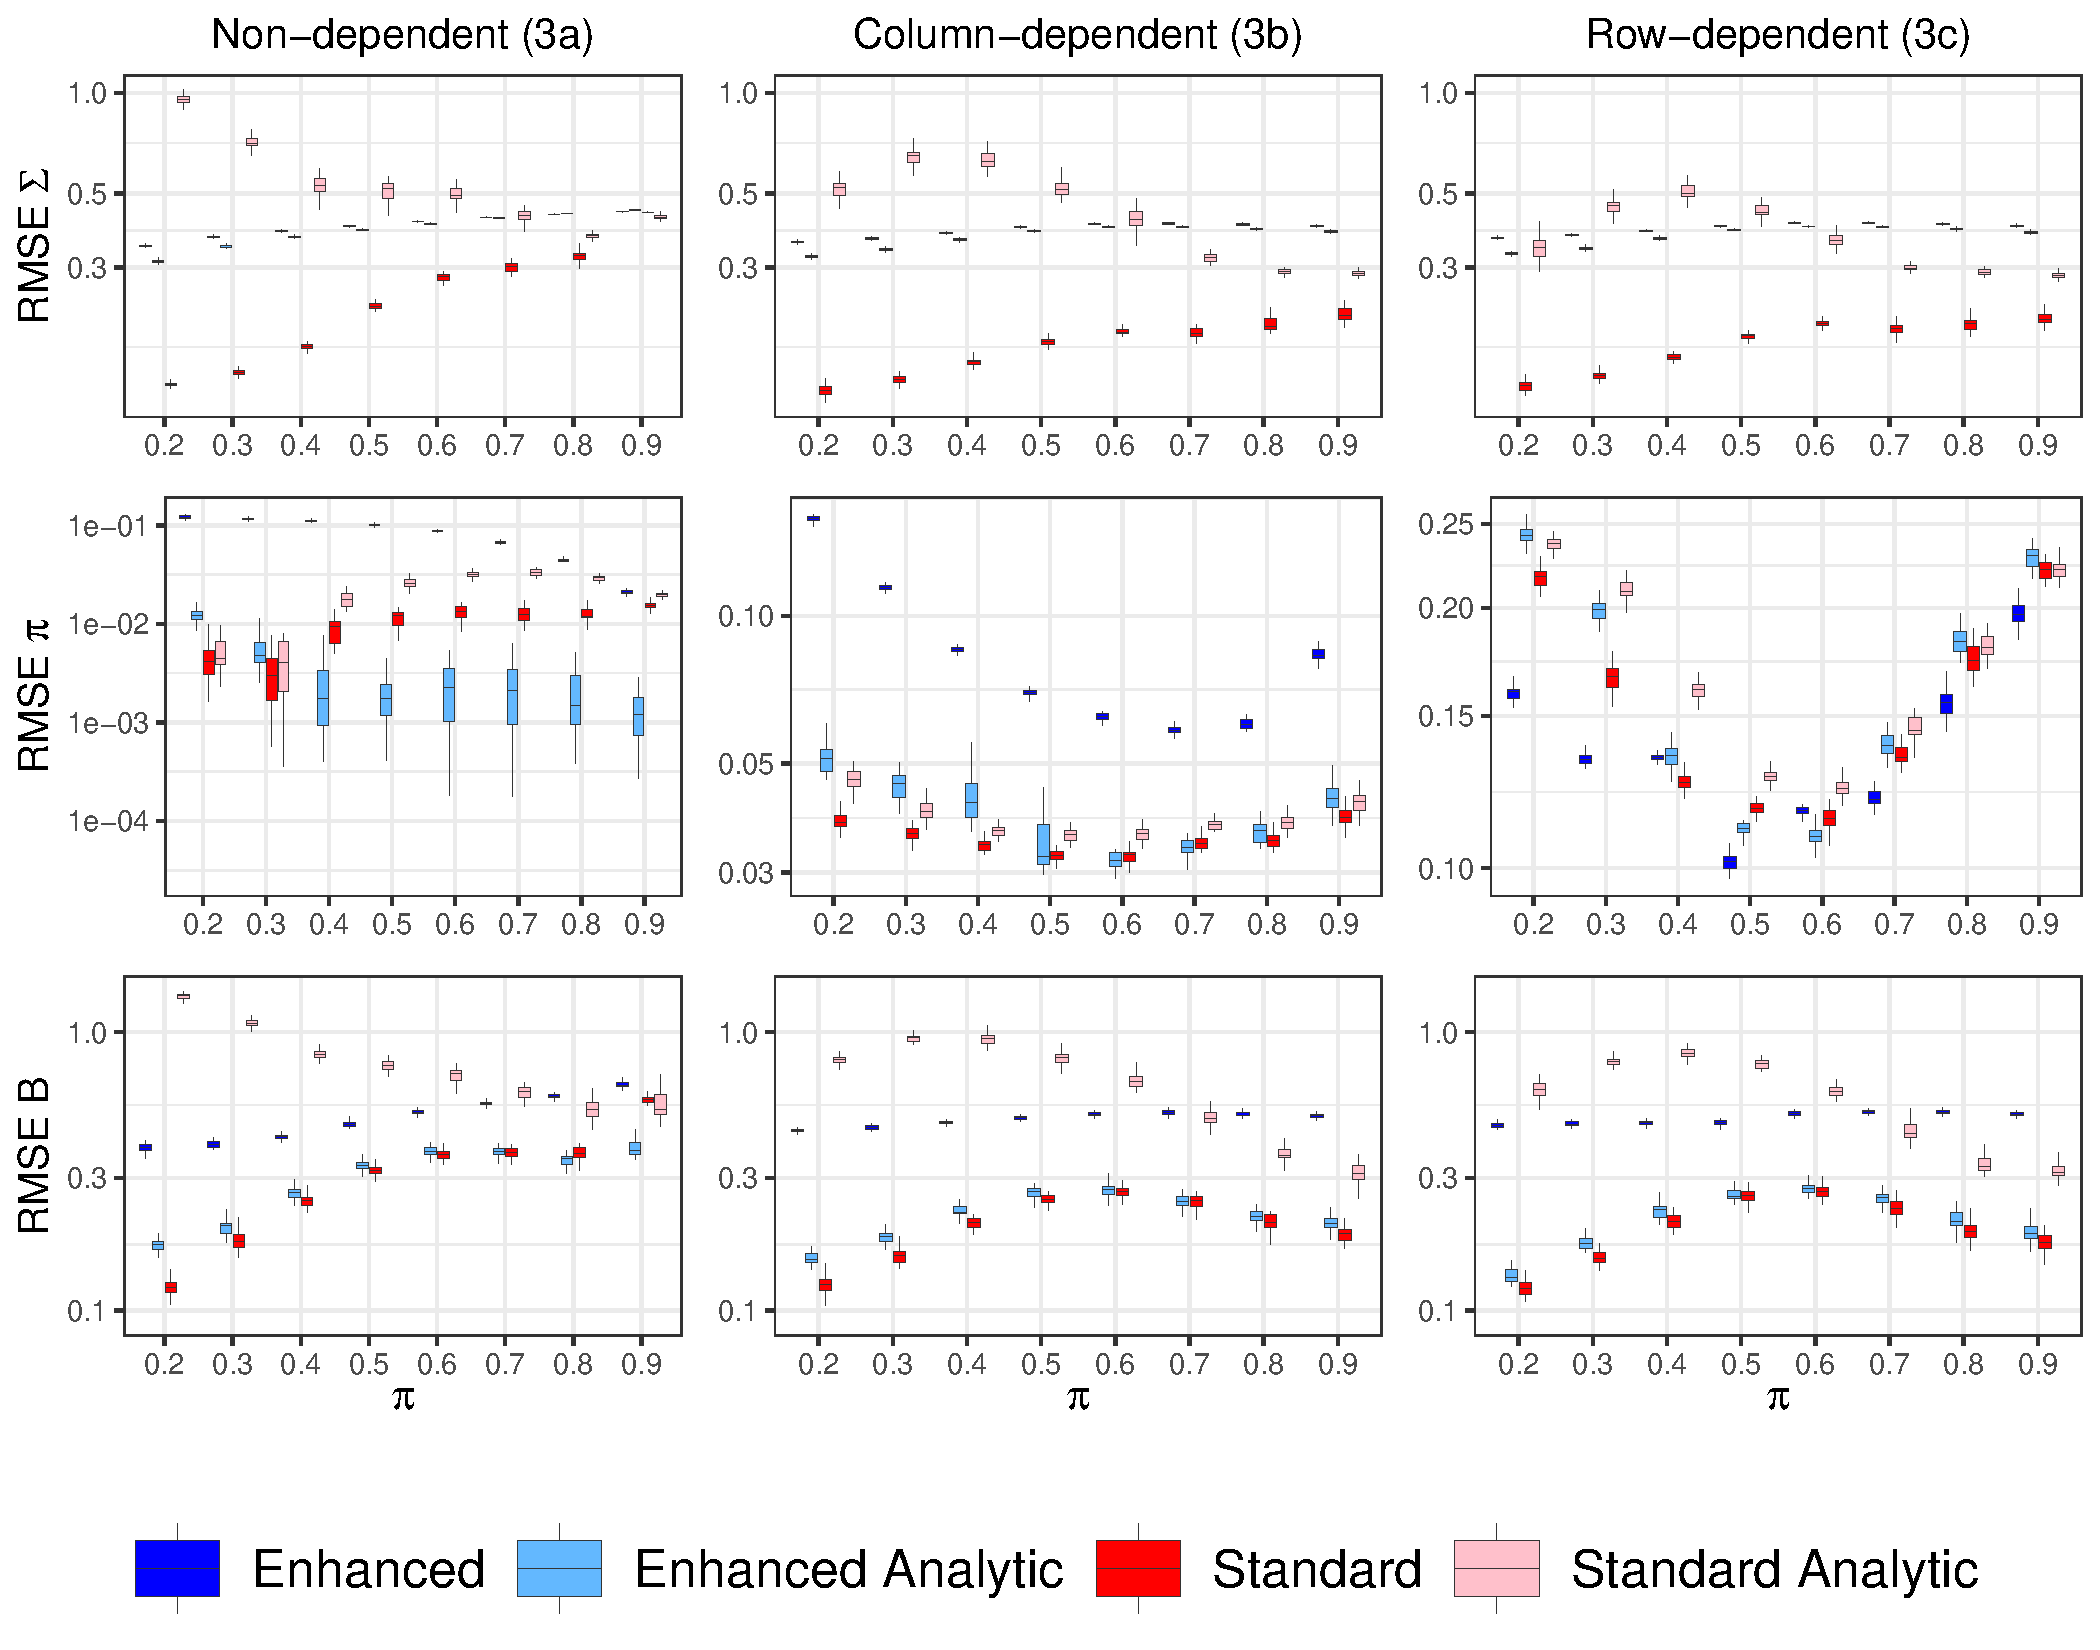
\includegraphics[scale=0.35]{figures/proba_stat.pdf}
\end{frame}
\begin{frame}{Applications on real data: ZIPLN vs PLN}
    \begin{itemize}
        \item
    \end{itemize}

\end{frame}
\end{document}

